\section{Implementation}
\subsection{Initialisation}
We set up a fully egalitarian generation. No person receives any inheritance. For the formation of consecutive generations, we explore the impact of several societal rules or patterns. We recognise:

\begin{itemize}
    \item Marital patterns: matchmaking of bachelors in function of inherited wealth
    \item Intestacy rules: either laws or habits that describe how bequeathed wealth is distributed among the children
\end{itemize}

In a single cycle, a generation of children turning adult receive an inheritance according to the input intestacy rules. All bachelors match according to the societal marital pattern following their bestowed wealth. The resulting couples optimise utility, and produce a next generation of children.

\subsection{Convergence}
Every generation produces a distribution of bequests $B_t$, leading to a distribution of inheritances $I_{t+1}$. In full equilibrium, subsequent generations experience the same distribution, or
\begin{equation}
    I_t = I_{t+1} = I^*
\end{equation}

We test for equality of two consecutive distributions by inspecting the \emph{Kolmogorov-Smirnov} statistic $D$. This measure is calculated as the largest difference observed in the two emperical distribution functions $F_{t,n}$ and $F_{t+1,n}$, or:
\begin{equation}
    D = \sup_x \left| F_{t,n}(x) - F_{t+1,n} \right|
\end{equation}

The Kolmogorov-Smirnov statistic follows, under the null hypothesis that both underlying distributions are equal, the Kolmogorov distibution. We can assess the p-values of the observed $D$ and infer the significance of the rejection of the null hypothesis in favour of inequality of distributions.

Not being able to reject the null hypothesis does not necessarily lead to "acceptation" of the null hypothesis. For now we follow the following pragmatic rule, that we consider the distributions safely converged, if we obtain a p-value greater than 50\% for five consecutive years.

\section{Results}
\subsection{Convergence}
Let us research the convergence of subsequent distributions. Figure \ref{fig:sfig1} shows the evolution of the p-value of the earlier mentioned Kolmogorov-Smirnov statistic $D$. We see that the threshold of five consecutive years above 50\% is somewhat arbitrary, but leads to a distribution that appears stationary apart from statistical noise. This is reflected in both the evolution of the Gini coefficient in figure \ref{fig:sfig2}, but also in the evolution of the underlying Lorentz curve. [hyperlink naar gif?]

\begin{figure}
\begin{subfigure}{\textwidth}
  \centering
  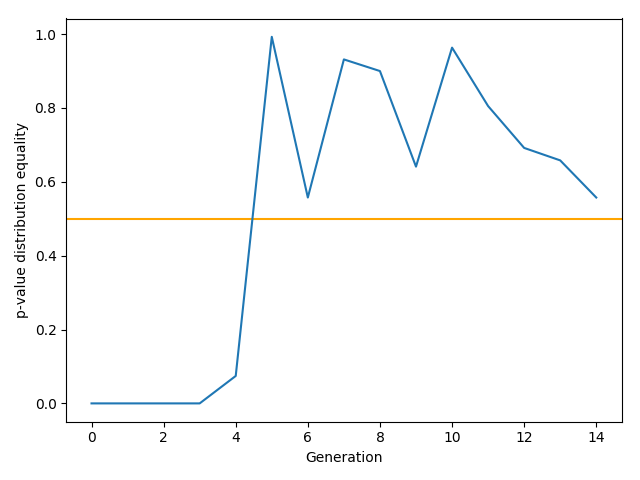
\includegraphics[width=.8\linewidth]{Results/images/P-value_ks_stat201803111436.png}
  \caption{Evolution of p-value of $D$ for consecutive distributions}
  \label{fig:sfig1}
\end{subfigure}\\
\begin{subfigure}{\textwidth}
  \centering
  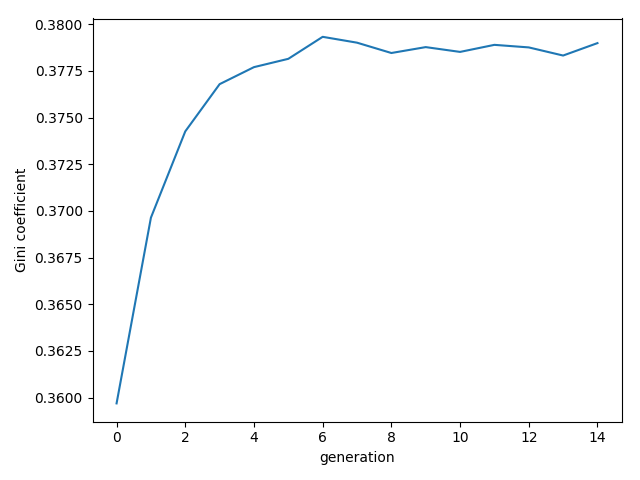
\includegraphics[width=.8\linewidth]{Results/images/gini_201803111436.png}
  \caption{Illustrative measure: evolution of the Gini coefficient. Notice it stabilises with a small noise}
  \label{fig:sfig2}
\end{subfigure}
\caption{Analysis of distribution convergence}
\label{fig:fig1}
\end{figure}

\subsection{Influence of societal patterns}
\label{sec:soc_pat}
For now we identify the following societal patterns:

\paragraph{Marital Patterns} We distinguish two extremes in the matching of bachelors. As discussed earlier, this comes down to:
\begin{itemize}
    \item Societies match bachelors by fully ordering all sets according to inherited wealth. (Class society)
    \item Bachelors are matched randomly. Inheritance plays no role
\end{itemize}

Let $\mathbf{i^M_t}$ be the vector containing all male individual inheritances (and likewise $\mathbf{i^F_t}$ for female inheritances), then in the class sociaty, the family inheritance vector $\mathbf{I_t}$ will be given by:
\begin{equation}
    \mathbf{I_t} = \mathbf{i^M_t}^\downarrow{} + \mathbf{i^F_t}^\downarrow{} 
\end{equation}
Where $\mathbf{X}^\downarrow{}$ denotes an ordered vector, from high to low.

In the case of random matching, family inheritance vectors are derived by
\begin{equation}
    \mathbf{I_t} = \mathbf{i_t^M} + P\mathbf{i_t^F}
\end{equation}
With $P$ a randomly chosen permutation matrix.

\paragraph{Intestacy rules}
Again we distinguish between two extremes:
\begin{itemize}
    \item Male-preference primogeniture. The eldest male child receives everything. In case there are no male heirs, the eldest female child receives all bequests
    \item Egalitarian inheritance. All children receive an equal part.
\end{itemize}

\paragraph{Comparison}

We apply several combinations of social patterns, and research the difference in Lorentz curves. The results are shown in figure \ref{fig:compare_gens}.
The striking conclusion is that in our model, said social patterns have an \emph{unambiguous} effect on wealth inequality: each Lorentz curve is fully contained within the next. This means that regardless of what measure of inequality we use, inequality is always found to be greatest in the class society with male primogeniture. The society with egalitarian inheritance and random matching is always the least unequal of the three considered sets. A society with egalitarian inheritance, but class bachelor matching is in between.

\begin{figure}
    \centering
    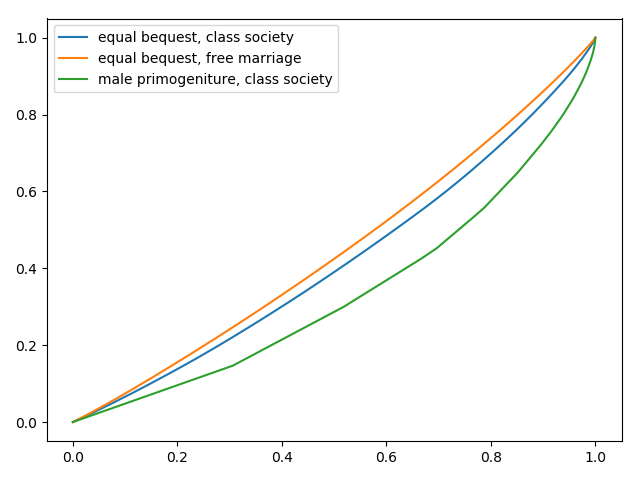
\includegraphics[width=0.8\linewidth{}]{Results/images/compare_rules.png}
    \caption{Lorentz curves for total family wealth after convergence for different combinations of societal patterns  }
    \label{fig:compare_gens}
\end{figure}

\section{Including a tax on inheritance}
\subsection{Proportional taxes}
Now we are ready to include a taxation on inherited wealth. We introduce the following system:
\begin{itemize}
    \item Upon reaching maturity and receiving their inheritance, all bachelors are taxed by a fraction $s$ of their inheritance. The total is divided among the population by a lump sum allowance $\mu$
    \item Parents optimise by $I_{t+1}^{net}$. In other words, the decision making process (\ref{eq:E}) remains unchanged
\end{itemize}

Let's introduce the society as in paragraph \ref{sec:soc_pat}, with class society marriage patterns, but egalitarian inheritance. We research the influence of taxation on inequality by calculating the converged Lorentz curve for different tax rates, from 0\% to 100\% with steps of 20 \%-point. Figure \ref{fig:prop_tax} shows the results.

Figure \ref{fig:prop_tax} shows that increasing an inheritance tax level decreases inequality in all strata of the population. If we quantify this inequality by the GINI coefficient, we see a gradual decline in figure \ref{fig:prop_gini}.

\begin{figure}
\begin{subfigure}{\textwidth}
  \centering
    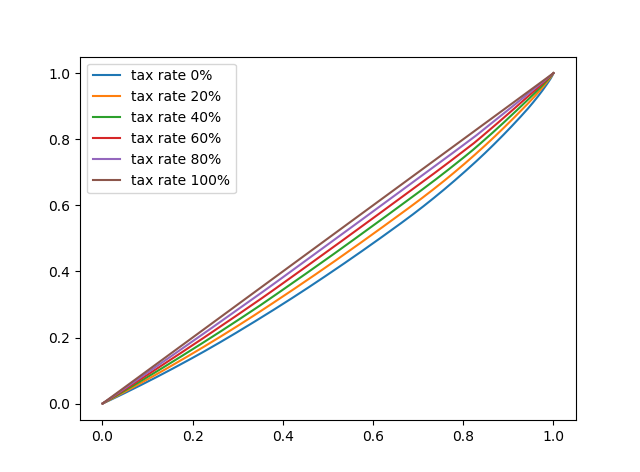
\includegraphics[width=0.9\linewidth]{Results/images/Figure_1.png}
    \caption{Lorentz curves for a class society with egalitarian inheritance for different proportional tax rates.}
    \label{fig:prop_tax}
\end{subfigure}\\
\begin{subfigure}{\textwidth}
  \centering
  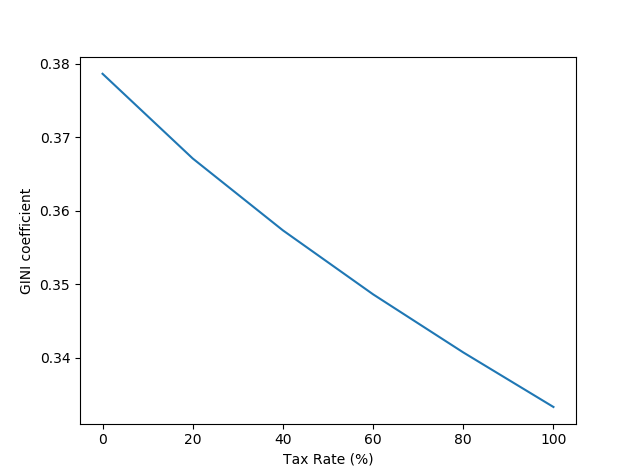
\includegraphics[width=.8\linewidth]{Results/images/GINI_prop.png}
  \caption{GINI coefficient under different tax rates}
  \label{fig:prop_gini}
\end{subfigure}
\caption{Analysis of effect of a proportional tax on inequality}
\label{fig:fig1}
\end{figure}

What is the influence of this taxation rate on employment? -> figure \ref{fig:prop_e}. Interesting to look into this?

\begin{figure}
    \centering
    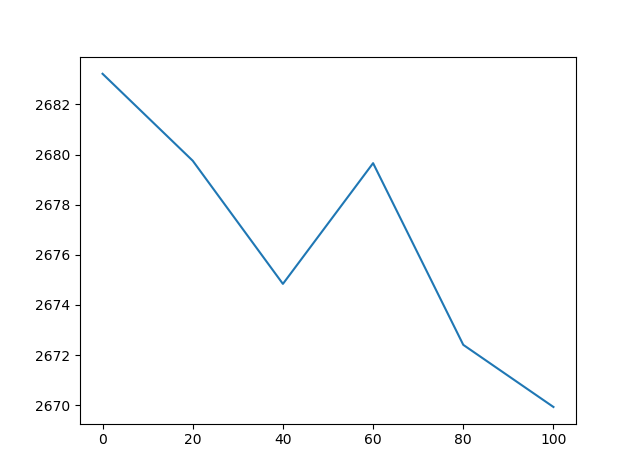
\includegraphics{Results/images/Figure_2.png}
    \caption{Total employment after convergence for different tax rates}
    \label{fig:prop_e}
\end{figure}